\section{Planificación del Trabajo}

\subsection{Descripción del grupo de trabajo}
A continuación se especificará el grupo de trabajo, el cual estará encargado del desarollo de la aplicación de conquista de espacios turísticos en 360°. Se especificará su ID, nombre, conocimientos, rol y contacto de cada uno de los integrantes del grupo de trabajo.

\begin{table}[H]
    \centering
        \begin{tabular}{|l | p{12cm} |}        
        \hline
        \textbf{ID} & FD \\
        \hline
        \textbf{Nombre} & Felipe Durán \\
        \hline
        \textbf{Conocimientos} & Experiencia en lenguaje de programación como Phython, C, C++, C\# , Java, JavaScript, Kotlin y Conocimientos con base de datos MySQL. \\
        \hline
        \textbf{Rol} & Planificador y Programador de la aplicación movil. \\    
        \hline
        \textbf{Contacto} & fduran16@alumnos.utalca.cl \\
        \hline            
        \end{tabular}
    \caption{Descripción Personal FD}
\end{table}


\begin{table}[H]
    \centering
        \begin{tabular}{|l | p{12cm} |}        
        \hline
        \textbf{ID} & IG \\
        \hline
        \textbf{Nombre} & Ignacio Gajardo \\
        \hline
        \textbf{Conocimientos} & Experiencia en lenguaje de programación como Phython, C, C++, C\# , Java, JavaScript, Kotlin y Conocimientos con base de datos MySQL. \\
        \hline
        \textbf{Rol} & Planificador y Programador de la aplicación movil. \\    
        \hline
        \textbf{Contacto} & igajardo16@alumnos.utalca.cl \\
        \hline            
        \end{tabular}
    \caption{Descripción Personal IG}
\end{table}


\begin{table}[H]
    \centering
        \begin{tabular}{|l | p{12cm} |}        
        \hline
        \textbf{ID} & AM \\
        \hline
        \textbf{Nombre} & Alex Molina \\
        \hline
        \textbf{Conocimientos} & Experiencia en lenguaje de programación como Phython, C, C++, C\# , Java y Conocimientos con base de datos MySQL. \\
        \hline
        \textbf{Rol} & Planificador y Programador de la aplicación movil. \\    
        \hline
        \textbf{Contacto} & amolina16@alumnos.utalca.cl \\
        \hline            
        \end{tabular}
    \caption{Descripción Personal AM}
\end{table}

Los recursos que se utilizarán en el desarrollo del proyecto del software de conquista de espacios turísticos en 360° son:

\begin{table}[H]
    \centering
        \begin{tabular}{|l | p{12cm} |}        
        \hline
        \textbf{ID} & FD\_Notebook \\
        \hline
        \textbf{Tipo de dispositvo} & Notebook \\
        \hline
        \textbf{Sistema operativo} & Window 10 Home \\
        \hline
        \textbf{Modelo} & Asus \\
        \hline
        \textbf{Procesador} & AMD FX-9830P RADEON R7 \\    
        \hline            
        \end{tabular}
    \caption{Recurso FD\_Notebook}
\end{table}


\begin{table}[H]
    \centering
        \begin{tabular}{|l | p{12cm} |}        
        \hline
        \textbf{ID} & IG\_Notebook \\
        \hline
        \textbf{Tipo de dispositvo} & Notebook \\
        \hline
        \textbf{Sistema operativo} & Window 10 Home \\
        \hline
        \textbf{Modelo} & MSI \\
        \hline
        \textbf{Procesador} & Intel Core i7-6700 \\    
        \hline            
        \end{tabular}
    \caption{Recurso IG\_Notebook}
\end{table}

\begin{table}[H]
    \centering
        \begin{tabular}{|l | p{12cm} |}        
        \hline
        \textbf{ID} & AM\_Notebook \\
        \hline
        \textbf{Tipo de dispositvo} & Notebook \\
        \hline
        \textbf{Sistema operativo} & Window 10 Home \\
        \hline
        \textbf{Modelo} & HP \\
        \hline
        \textbf{Procesador} & Intel Core i5-7300 \\    
        \hline            
        \end{tabular}
    \caption{Recurso AM\_Notebook}
\end{table}

\subsection{Estimación de esfuerzo}
Se a realizado un analisis de todos los aspectos posibles que serán parte del desarrollo del software y que competen a la estimación de esfuerzo. Sin embargo, todo lo analizado queda sujeto a modificaciones, debido principalmente a que el proyecto está aún en desarrollo y no se encuentra una versión base o una visión profesionalmente detallada de las iteraciones para desarrollar el producto final. Tanto a nivel de programación como de diseño a de ser necesaria una frecuente revisión y actualización con cada iteración y avance en este proyecto.

Según lo conversado, pactado y analizado con el equipo de desarrollo en la primera iteración, el análisis del proyecto se puede apreciar en las siguientes graficas de estimación de puntos de esfuerzo.
\begin{figure}[htbp]
	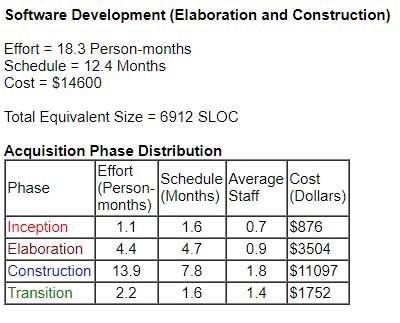
\includegraphics{imgs/1.JPG}
	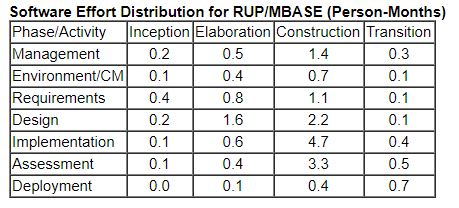
\includegraphics[scale=0.9]{imgs/2.JPG}
\end{figure}

\begin{figure}[htbp]
	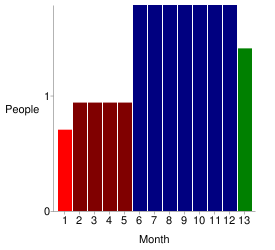
\includegraphics{imgs/Grafica.png}
	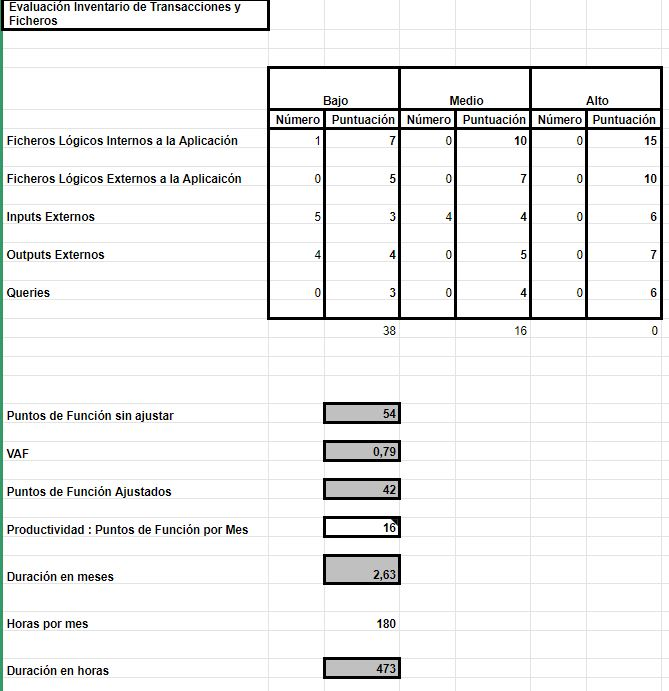
\includegraphics[scale=0.5]{imgs/Estimacion de PF.JPG}
\end{figure}

\subsection{Asignación de recursos}
\begin{table}[H]
    \begin{center}
        \begin{tabular}{| l | m{12cm} |}        
        	\hline 
        	Recurso & Asigando a \\
        	\hline
        	Felipe Duran & Encargado de programación, FD\_Notebook\\
        	\hline
        	Alex Molina & Encargado de administración, AM\_Notebook\\
        	\hline
        	Ignacio Gajardo & Encargado de diseño, IG\_Notebook\\
        	\hline
        \end{tabular}
    \caption{Asignacion del personal a sus distintos cargos}
    \end{center}
\end{table}
\subsection{Planificación temporal de actividades}

\textbf{Gráficos de la planificación actual:}

\begin{figure}[htbp]
	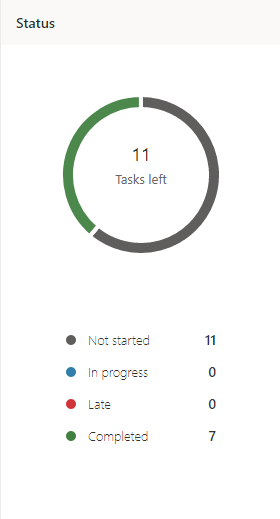
\includegraphics[scale=0.7]{imgs/planner_status.png}
	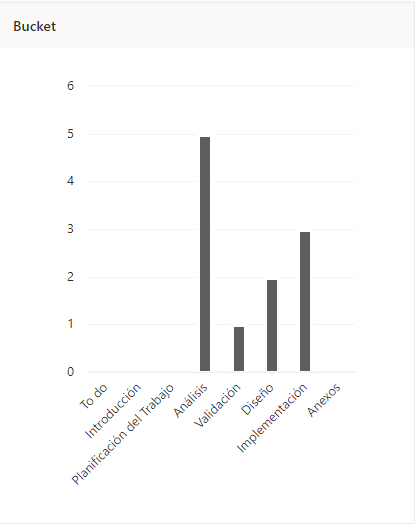
\includegraphics[scale=0.7]{imgs/planner_bucket.png}
\end{figure}

\begin{figure}[htbp]
	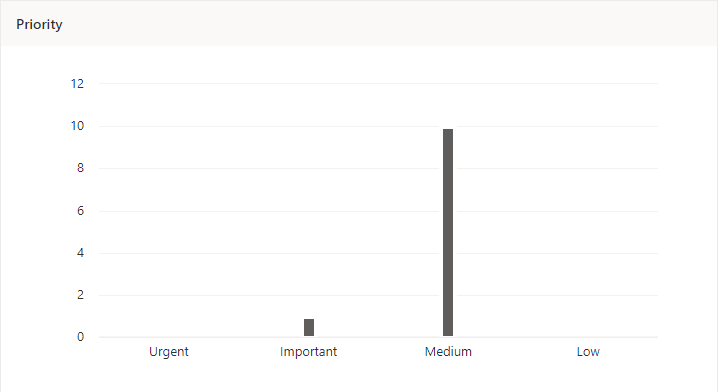
\includegraphics[scale=0.7]{imgs/planner_priority.png}
	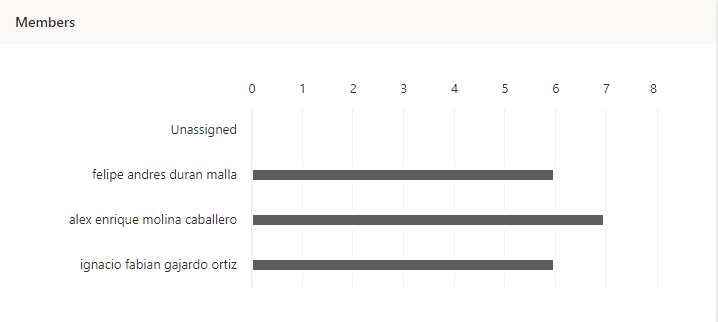
\includegraphics[scale=0.7]{imgs/planner_members.png}
\end{figure}